\documentclass[runningheads]{llncs}
%

\usepackage{amsmath}
\usepackage{amsfonts}
%\usepackage{amsthm}

\usepackage{tabularx}
\usepackage{graphicx}
\usepackage{hyperref}

\usepackage{float}
\usepackage{array}
\usepackage{mdframed}
\usepackage{tikz}
\usepackage{placeins}

\graphicspath{{figures/}}




\usepackage{algorithm}
\usepackage{algpseudocode}
\makeatletter
\algrenewcommand\ALG@beginalgorithmic{\fontsize{10pt}{2cm}}
\makeatother

\algnewcommand\algorithmicpublicinput{\textbf{Public input:}}
\algnewcommand\Public{\item[\algorithmicpublicinput]}

\algnewcommand\algorithmicprivateinput{\textbf{Private input:}}
\algnewcommand\Private{\item[\algorithmicprivateinput]}



\usepackage[document]{ragged2e}


\usetikzlibrary{math}
\usetikzlibrary{arrows.meta}



\newfloat{Protocol}{t}{struct}

\newfloat{circuit}{t}{loa}
\floatname{circuit}{Circuit}

\newfloat{contractfunction}{t}{loa}
\floatname{contractfunction}{Rollup contract function}

\usepackage[nameinlink]{cleveref}

\Crefname{circuit}{Circuit}{Circuits}
\Crefname{contractfunction}{Rollup contract function}{Rollup contract functions}

\newtheorem{defn}{Definition}
\newtheorem{prop}{Proposition}
\newtheorem{cor}{Corollary}


% Used for displaying a sample figure. If possible, figure files should
% be included in EPS format.
%
% If you use the hyperref package, please uncomment the following line
% to display URLs in blue roman font according to Springer's eBook style:
%\renewcommand\UrlFont{\color{blue}\rmfamily}

\begin{document}
%
\title{
Intmax2: A ZK-rollup with Minimal Onchain Data and Computation Costs Featuring Decentralized Aggregators
}
%
\titlerunning{Intmax2}
% If the paper title is too long for the running head, you can set
% an abbreviated paper title here
%
%\author{
%Erik Rybakken\inst{1} 
%\and
%Leona Hioki\inst{1}
%\and
%Mario Yaksetig\inst{2}
%}
\author{}
%
%\authorrunning{E. Rybakken et al.}
% First names are abbreviated in the running head.
% If there are more than two authors, 'et al.' is used.
%
%\institute{
%Intmax
%\\
%\email{paper@intmax.io}
%\and
%University of Porto
%}
\institute{}
%
\maketitle              % typeset the header of the contribution
%
\begin{abstract}
We present a novel blockchain scaling solution called Intmax2, which is a Zero-Knowledge rollup (ZK-rollup) protocol featuring stateless and decentralized block production, while minimizing the usage of data and computation on the underlying blockchain. Our architecture distinctly diverges from existing ZK-rollups since essentially all of the data and computational costs are shifted to the client-side as opposed to imposing heavy requirements on the block producers or the underlying Layer 1 blockchain. The only job for block producers is to periodically generate a commitment to a set of transactions, distribute inclusion proofs to each sender, and collect and aggregate signatures by the senders. This design allows permissionless and stateless block production, and is highly scalable with the number of users.
\keywords{Zero-Knowledge Proofs  \and Stateless ZK-Rollup \and Blockchain Scaling}
\end{abstract}
%
%
%

% Introduction
\section{Introduction}
    As the blockchain ecosystem continually evolves, so does the urgency for blockchain scaling solutions that preserve security, reduce transaction costs, and improve overall throughput. Layer 2 (L2) technologies, particularly rollups, have emerged as pivotal tools to overcome these challenges, and have thus gathered substantial attention. Among these, Zero-Knowledge rollups (or ZK-rollups) have shown great promise due to their unique capability to bundle numerous transactions into a single proof that can be verified quickly and cheaply onchain. Existing ZK-rollups, while managing to move computation costs away from the underlying Layer 1 (L1) blockchain, are still limited by the fact that all necessary data for verifying users' balances have to be posted on L1. This data, in a typical scenario, includes the transaction sender, the index of the token, the amount, and the recipient for each transaction, thus limiting the number of transactions per second that can be supported by the rollup.

\subsection{Data Availability}

A fundamental bottleneck for blockchains is what is known as data availability. Data availability means that transaction data needs to be available in order to be able to prove the current state, such as account balances, of the blockchain. This is a problem for both Layer 1 blockchains and rollups. Layer 1 blockchains usually achieve data availability by requiring that all transaction data is publicly available for a node to consider the blockchain valid. Rollups achieve data availability by leveraging the data availability of the underlying blockchain and require that all transaction data is posted to L1 (e.g. using calldata or blob data on Ethereum). Because this data needs to be replicated among a large set of nodes, there is a limit on how much data can be made available, which limits the number of transactions per second that the blockchain or the rollup can support. While for smart contract blockchains it might be necessary to provide the complete transaction data, it turns out that for simple payment transactions it is only necessary to make available a commitment to the set of transactions in a block (such as a Merkle tree root), together with the set of senders who have signed the commitment, confirming that they have received inclusion proofs of their transactions. Users can then generate Zero-Knowledge proofs (ZK-proofs) of their own balances by combining the inclusion proofs of their sent transactions with the inclusion proofs and ZK-proofs of sufficient balance of each received transaction, which is provided by the transaction sender offchain. Our rollup design uses this method to achieve increased throughput compared to existing alternatives. In addition, the design allows permissionless block building that can happen in parallel, without needing any leader election or any coordination between the block builders. Since the block builders do not verify the validity of the transactions, they can be fully stateless, allowing a very simple and censorship resistant rollup design.

\subsection{Our Contributions}

Intmax2 is an efficient and stateless rollup design that:

\begin{itemize}
  \setlength\itemsep{0.35em}

    \item Uses less onchain data than any existing rollup, giving an upper limit of 7500 transaction batches per second on Ethereum, where each transaction batch can transfer an unlimited number of tokens to an unlimited number of recipients.

    % %MY: maybe change phrasing
    % \item Shifts the computational requirements from the aggregator to the client, making it highly scalable with the number of users.

    \item Offers permissionless block production.

    \item Provides stronger privacy properties than traditional ZK-rollups.
  
\end{itemize}

\subsection{Formal verification of the security proof}

We give a pen-and-paper proof of the security of the protocol in \Cref{thm:rollup-contract-is-secure}. This proof has been formally verified in the Lean theorem prover\cite{demoura2021the} by the Nethermind Formal Verification team \cite{nethermind}. All mathematical definitions and statements that are needed for the security proof contain a hyperlink (like this: \href{https://github.com/\repo FVIntmax/}{\ExternalLink}) to the formalized version.

\section{Preliminaries}
    



%\section{Important Definitions}
    \section{Simplified design description}\label{section:simplified-design}

In this section we describe a simplified version of the design which
doesn't use ZK-proofs. The simplified design achieves low onchain
data consumption (4-5 bytes per transaction sender), but is otherwise
inefficient and not private. In \Cref{section:zk} we add ZK-proofs to
the design in order to achieve efficiency and privacy.

\subsection{Overview}

The simplified design works roughly as follows. At the heart of the
design is a rollup contract deployed on a programmable blockchain
(such as Ethereum). To deposit funds to the rollup, a user simply
sends the funds, together with the L2 address of the recipient, to
the rollup contract which then records the deposit in its contract
storage. To transfer funds on the rollup, a subset of L2 accounts
will first send their transactions to a single aggregator, which then
inserts the transactions at the leaves of a merkle tree. Then the
aggregator sends to each sender the merkle root and the merkle proof
for that sender's transaction. Each sender then signs the merkle root
with their public BLS key and sends this signature back to the
aggregator. The aggregator then aggregates the signatures into a
single aggregated signature, and sends the merkle root, the
aggregated signature and the list of public keys of the senders that
was included in the aggregated signature to the rollup contract. The
rollup contract then verifies the signature and adds the root,
signature and sender list to its storage. Each sender is then
responsible for sending the merkle proof of the transaction to each
transaction recipient offchain, together with earlier merkle proofs
that together prove that the sender had sufficient balance for the
transaction. To prove their own balance, each user needs to keep
track of all merkle proofs they have received from aggregators and
other users. This collection of merkle proofs, called a balance
proof, is sent to the rollup contract when a user wants to withdraw
their funds to L1.

We now describe the simplified design in more details.

\subsection{Notation}

If \(X\) and \(Y\) are sets, we will write \(Y^X\) for the set of all
functions from \(X\) to \(Y\). We will often call a function \(f \in
Y^X\) a \emph{mapping} from (elements of) \(X\) to (elements of) \(Y\).

\subsection{Setup}

The design depends on an authenticated dictionary scheme\footnote{See
\Cref{section:authenticated-dictionaries}.} \(\mathsf{AD}\), a
signature aggregation scheme\footnote{See
\Cref{section:signature-aggregation}.} \(\mathsf{SA}\), and a
collision-resistant hash function \(\mathsf{H} : \{0,1\}^* \to
\{0,1\}^n\). Given a security parameter \(\lambda \in \N\) we set up
the authenticated dictionary scheme
\[\mathsf{AD}.(\K,\M,\C,\Pi,\mathsf{Commit},\mathsf{Verify})\] and
the signature aggregation scheme \[\mathsf{SA}.(\K_p, \K_s, \Sigma,
    \mathsf{KeyGen}, \mathsf{Sign}, \mathsf{Aggregate},
\mathsf{Verify}).\] We use the alias \(\K_2 := \mathsf{SA}.\K_p\) and
call this the set of \emph{L2 accounts}. We also depend on a set
\(\K_1\) of L1 accounts\footnote{For instance, in Ethereum, accounts
  are represented by 20 bytes, so in this case we have \(\K_1 :=
\{0,1\}^{20\cdot8}\).}, and a lattice-ordered abelian group \(\V\)
which is used as the set of transaction values and account
balances.\footnote{See \Cref{section:lattice-ordered-abelian-groups}
  for the definition of a lattice-ordered abelian group. This
  generality allows us to easily support transfers of multiple value
  types (e.g. NFTs, ERC20 tokens, etc.) by letting \(\V\) be the set of
  mappings from a set of token names to the set \(\Z\) of integers,
  which naturally gets the structure of a lattice-ordered abelian
group.} We denote by \(\V_+ \subseteq \V\) the subset of positive
values, defined as the values \(v \in \V\) where \(v \geq 0\).

\subsection{Rollup contract}

The rollup contract is a smart contract deployed on a programmable
blockchain (e.g. Ethereum), which is responsible for keeping track of
the rollup state and for managing deposits, transfers, and
withdrawals. The internal state of the rollup contract consists of
the list of all blocks that have been added to the rollup so far.
There are three types of blocks in our design, namely deposit blocks,
transfer blocks and withdrawal blocks, denoted by \(\B_{deposit}\),
\(\B_{transfer}\) and \(\B_{withdrawal}\) respectively. We formally
define these sets below where we describe the respective protocols.
Letting \(\B := \B_{deposit} \amalg \B_{transfer} \amalg
\B_{withdrawal}\) be the set of all blocks
\href{https://github.com/\repo
FVIntmax/Block.lean#L14}{\ExternalLink}, the contract state is
formally defined \href{https://github.com/\repo
FVIntmax/Block.lean#L115}{\ExternalLink} as \[\S_{contract} :=
\B^*.\] When the rollup contract is deployed to the blockchain, it is
initialized with the state \(()\) consisting of the empty list
\href{https://github.com/\repo FVIntmax/Block.lean#L125}{\ExternalLink}.

\subsection{Depositing}\label{section:depositing}

To deposit funds from L1 to L2, a L1 user will simply send the funds
to the rollup contract along with the L2 address of the recipient.
The rollup contract then constructs a \emph{deposit block} which
consists of the specified recipient and the deposited amount.
Formally, we define \href{https://github.com/\repo
FVIntmax/Block.lean#L18}{\ExternalLink} the set of deposit blocks as
\[\B_{deposit} := \K_2 \times \V_+.\] The contract then adds this
deposit block to the list of blocks in its storage.

\subsection{Transferring}\label{section:transferring}

We now describe the protocol for transferring funds on the rollup
(illustrated in \Cref{fig:user-protocol}). To transfer funds from an
L2 account, the account owner will first construct a
\emph{transaction batch}, which is a mapping that maps each
transaction recipient to the amount the sender wants to send to that
recipient. A transaction recipient is either an L2 account or an L1
account (used when withdrawing to L1, as described in
\Cref{section:withdrawing}). Formally, letting \(\K := \K_1 \amalg
\K_2\) \href{https://github.com/\repo
FVIntmax/Key.lean#L14}{\ExternalLink}, a transaction batch is an
element of \(\V_+^{\K},\) i.e. a mapping from \(\K\) to \(V_+\)
\href{https://github.com/\repo
FVIntmax/TransactionBatch.lean#L22}{\ExternalLink}.

Suppose we have a set of senders \(S \subseteq \K_2\) where each
sender \(s \in S\) has a secret key \(sk_s\) and a transaction batch
\(t_s \in \V_+^{\K}\) they want to send. The transfer protocol
consists of two phases. In the first phase, the senders collaborate
with a single aggregator to produce a \emph{transfer block} which is
added to the rollup contract. In the second phase, after the transfer
block has been added to the rollup contract, each transaction sender
\(s\) will send (offchain) to each recipient (i.e. accounts \(r \in
\K\) where \(t_s(r) \neq 0\)) the data needed to prove that the
sender sent the specified amount to the recipient in the transfer
block. We now describe the two phases of the transfer protocol in more details.

% \begin{itemize}
%   \item The L1 address \(aggregator \in \K_1\) of the aggregator.
%   \item A string \(extradata \in \{0,1\}^*\) that has been agreed
% upon by the senders and aggregator, which can be used to implement
% protection against replay attacks and delayed block publication
% (see \Cref{section:protection}).
%   \item An authenticated dictionary commitment \(C \in
% \mathsf{AD}.\C\) of a dictionary which maps each sender to the hash
% of their transaction batch (concatenated with a random salt chosen
% by the sender).

%   \item A subset of senders \(S' \subset \K_2\) that have received
% a lookup proof of their own transaction batch hash from the aggregator.
%   \item An aggregated signature \(\sigma \in \mathsf{SA}.\Sigma\)
% of the tuple \((aggregator, extradata, C)\) by the senders in \(S'\).
% \end{itemize}

% Formally, we define the set of transfer blocks as \[\B_{transfer} =
% \K_1 \times \{0,1\}^* \times \mathsf{AD}.\C \times \mathcal{P}(\K)
% \times \mathsf{SA}.\Sigma.\]

% In the second phase, after the transfer block has been added to the
% rollup contract, each transaction sender \(s\) will send (offchain)
% to each recipient (i.e. accounts \(r \in \K\) where \(t_s(r) \neq
% 0\)) the data consisting of the transaction batch \(t_s\), the salt
% used for the transaction batch hash, a lookup proof of
% \(\mathsf{H}(t_s,salt)\) in the dictionary commitment \(C\), and
% \emph{all transaction batches, salts and lookup proofs that the
% transaction sender has previously received}. All this data is
% needed to prove to the recipient that the sender has sufficient
% balance for the transaction. We now describe the two phases of the
% transfer protocol in more details.

\subsubsection{Phase 1: Constructing and adding a transfer
block}\label{section:transferring-phase-1}

To send the transaction batches, the senders will first select a
single aggregator\footnote{The protocol allows anyone to be an
  aggregator for a transfer block, enabling maximum censorship
resistance.} and agree upon a common bitstring \(extradata \in
\{0,1\}^*\). This bitstring can be used to implement protections
against replay attacks and delayed block publication (see
\Cref{section:protection}). Then the senders and aggregator interacts
in the following protocol.

\begin{enumerate}
  \item First, each sender \(s\) chooses a random salt \(salt_s\),
    hashes their transaction batch with the salt \[h_s \leftarrow
    H(t_s,salt_s),\] and sends \(h_s\) to the
    aggregator.\footnote{Sending the transaction hash instead of the
    transaction itself gives privacy from the aggregator.}
  \item The aggregator collects all the transaction batch hashes from
    the senders. Let \(S' \subseteq S\) be the subset of senders who
    sent a transaction batch hash to the aggregator. The aggregator
    then constructs the dictionary\footnote{See
    \Cref{section:dictionaries} for the definition of a dictionary.}
    \((S',h)\) where \(h_s\) is the transaction batch hash by \(s\)
    for all \(s \in S'\), and constructs a dictionary commitment and
    lookup proofs: \[(C, (S',\pi)) \leftarrow
    \mathsf{AD.Commit}(S',h).\] The aggregator sends to each sender
    \(s \in S'\) the dictionary commitment \(C\) and the lookup proof
    \(\pi_s\) for the sender's transaction batch hash.
  \item Upon receiving the dictionary commitment and lookup proof,
    each sender \(s\) checks if the lookup proof is valid with the
    commitment: \[\mathsf{AD.Verify}(\pi_s,s,h_s,C) \stackrel{?}{=}
    True.\] If the lookup proof is valid, the sender generates the
    signature \[\sigma_s \leftarrow
    \mathsf{SA.Sign}(sk_s,(C,aggregator,extradata))\] and sends this
    signature to the aggregator.
  \item The aggregator collects the signatures from the senders and
    verifies them. Let \(S'' \subseteq S'\) be the subset of senders
    who sent a valid signature. The aggregator then constructs the
    aggregated signature \[\sigma \leftarrow
    \mathsf{SA.Aggregate}((s,\sigma_s)_{s \in S''}),\] and constructs
    the tuple \((aggregator,extradata,C,S'',\sigma)\), called a
    \emph{transfer block}. Formally, we define the set of transfer
    blocks \href{https://github.com/\repo
    FVIntmax/Block.lean#L25}{\ExternalLink}as \[\B_{transfer} = \K_1
      \times \{0,1\}^* \times \mathsf{AD}.\C \times \mathcal{P}(\K_2)
    \times \mathsf{SA}.\Sigma.\]
    The aggregator sends this transfer block to the rollup contract
    using their L1 account.
  \item Upon receiving the transfer block, the rollup contract
    verifies the aggregated signature:
    \[\mathsf{SA.Verify}(S'',(C,aggregator,extradata),\sigma)
    \stackrel{?}{=} True\] and also verifies that the transaction is
    indeed coming from the account \(aggregator\). If these checks
    are valid, the contract adds the transfer block to the list of
    blocks in its storage. If not, the transaction is reverted.
\end{enumerate}

\begin{figure}

  \centering
  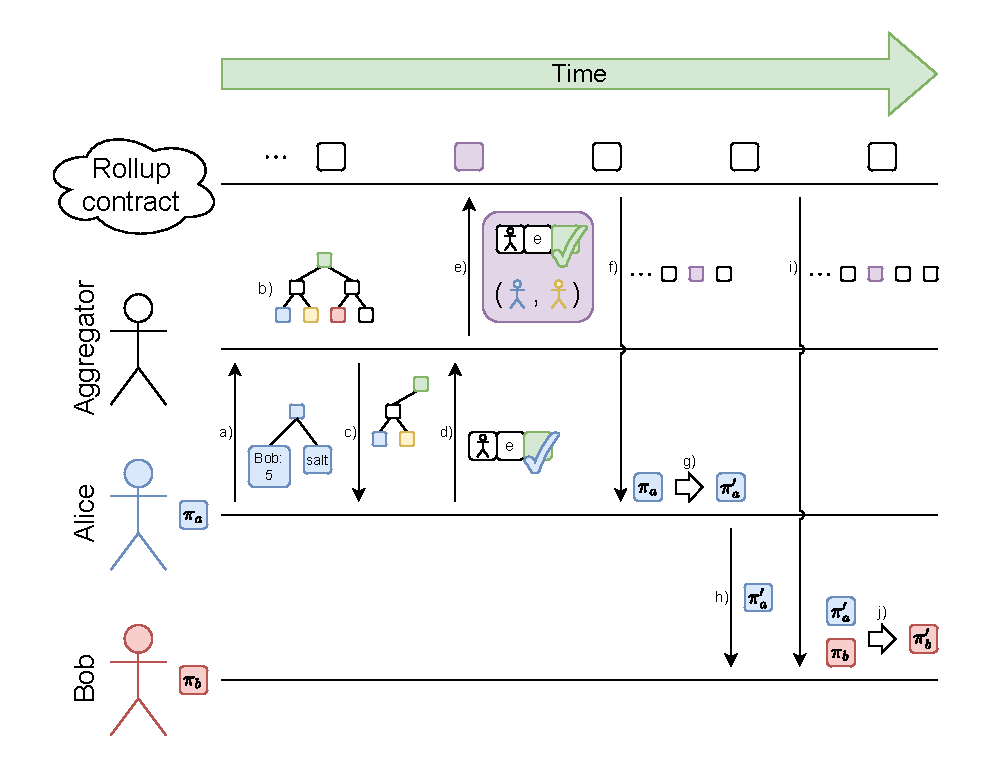
\includegraphics[width=\textwidth]{user-protocol.pdf}
  \caption{The transfer protocol. In this example, Alice wants to send
  5 coins to Bob. a) Alice starts by sending the hash of the the
  transaction batch, consisting of a single transaction of 5 coins to
Bob, and a random salt to an aggregator. b) The aggregator then
constructs a merkle tree consisting of Alice's transaction batch hash
and the transaction batch hashes of other senders. c) The aggregator
sends the merkle proof of Alice's transaction batch to Alice. d)
Alice verifies the merkle proof and signs the merkle root together
with the pre-determined extradata \(e\). This signature is sent back
to the aggregator. e) The aggregator collects the signatures from all
senders, constructs the transfer block, and sends it to the rollup
contract. f) Alice watches the blocks that are added to the rollup
contract until the block containing her transaction is published. g)
Alice updates her balance proof by adding her transaction batch, the
salt and the merkle proof. h) Alice sends to Bob her updated balance
proof. h) Bob updates his view of the rollup blocks. i) Bob updates
his balance proof by merging it with the balance proof he received from Alice.}
\label{fig:user-protocol}
\end{figure}

\subsubsection{Phase 2: Maintaining and distributing balance proofs}

To be able to prove the balance of their account, each user needs to
maintain a \emph{balance proof}, which is the collection of
transaction batches with corresponding salts and lookup proofs that
they have received from an aggregator (when sending transactions) and
from other users (when receiving transactions). We formally define
\href{https://github.com/\repo
FVIntmax/BalanceProof.lean#L27}{\ExternalLink} the set of balance
proofs as \[\Pi := Dict(\mathsf{AD}.\C \times \K_2, (\mathsf{AD}.\Pi
\times \{0,1\}^*) \times \V_+^{\K}).\]

A balance proof is valid if the following algorithm returns \(True\)
\href{https://github.com/\repo FVIntmax/BalanceProof.lean#L60}{\ExternalLink}.
\[
\begin{aligned}[t]
\mathsf{Verify} \colon \Pi & \to \{True,False\}                       \\
(K,D)                      & \mapsto \bigwedge_{\substack{(C,s) \in K
\\ ((\pi,salt), t) = D(C,s)}} \mathsf{AD.Verify}(\pi,s,\mathsf{H}(t,salt),C)
\end{aligned}\]

In other words, a valid balance proof is a dictionary which maps
commitment-sender pairs \((C,s)\) to tuples \(((\pi,salt), t)\) where
\(t \in \V_+^{\K}\) is a transaction batch, \(salt\) is a random salt
and \(\pi \in \mathsf{AD}.\Pi\) is a valid lookup proof that
\(H(t,salt)\) is the value at index \(s\) in an authenticated
dictionary with commitment \(C\).

Each user will maintain a balance proof, which is initialized as the
empty dictionary. In the second phase of the transfer protocol, each
transaction sender will add their transaction batch with the
corresponding lookup proof they received from the aggregator (if they
did receive one) to their own balance proof. Then, they will send
this new balance proof to each recipient of the transaction batch.
Upon receiving the balance proof, each recipient will then merge it
with their own. In details, if \(\pi_b \in \Pi\) is the current
balance proof of a recipient named Bob and \(\pi_a \in \Pi\) is the
balance proof they received from a sender named Alice, then Bob
performs the following algorithm:

\begin{itemize}
\item Verify the received balance proof: \[\mathsf{Verify}(\pi_a)
\stackrel{?}{=} True.\] If valid, continue to the next step,
otherwise terminate.
\item Update their balance proof \(\pi_b\) by merging it with
\(\pi_a\): \[\pi_b \leftarrow \mathsf{Merge}(\pi_a, \pi_b),\] where
\(\mathsf{Merge}\) is the dictionary merging algorithm defined in
\Cref{section:dictionaries}.
\end{itemize}

To compute the balance of their accounts, users will use the balance
function \[\mathsf{Bal} \colon \Pi \times \B^* \to \S,\] defined in
\Cref{section:balances}. Here \(\S\) is the set of states, where a
state is an assignment of a balance to each account. Formally, let
\(\overline{\K} := \K_1 \amalg \K_2 \amalg \{\source\}\), where
Source is a special account used to represent deposits and
withdrawals. Then the set of states \(\S\) is defined
\href{https://github.com/\repo
FVIntmax/State.lean#L31}{\ExternalLink}as \[\S := \{b \in
\V^{\overline{\K}}, \text{ such that } b_k \geq 0,\, \forall k \in
\overline{K}\backslash \{\source\}\}.\] The balance function takes a
balance proof \(\pi \in \Pi\) and the current state of the rollup
contract \((B_*) \in \B^*\), and returns the balance of each account
in the rollup that can be proven by the balance proof.

\subsection{Withdrawing}\label{section:withdrawing}

When a user wants to withdraw funds from their L2 account to an L1
account, they must first transfer the funds to the L1 account using
the transfer protocol described above. When the transfer block is
added to the rollup contract, the contract does not automatically
withdraw the funds to L1. Instead, to initiate the withdrawal, the
owner of the L1 account must send a withdrawal request to the rollup
contract which consists of the user's current balance proof \(\pi \in
\Pi\). Upon receiving the balance proof, the rollup contract performs
the following steps:

\begin{itemize}
\item First, the balance proof is verified: \[\mathsf{Verify}(\pi)
\stackrel{?}{=} True.\]
\item If the balance proof is valid, the rollup contract constructs a
withdrawal block, which is simply the in-rollup balance of each L1
account computed from the balance proof and the current rollup state:
\[B \leftarrow \mathsf{Bal}(\pi,B_*)\vline_{K_1},\] where \(B_*\) is
the current list of blocks in the rollup contract. Formally, the set
of withdrawal blocks is defined \href{https://github.com/\repo
FVIntmax/Block.lean#L31}{\ExternalLink}as \[\B_{withdrawal} = \V_+^{K_1}.\]
\item The contract adds the withdrawal block \(B\) to the list of
blocks in its storage: \[B_* \leftarrow (B_* || (B))\]
\item For each L1 account \(k \in K_1\), the contract withdraws the
amount \(B_k\) to the L1 account.
\end{itemize}

These steps ensure that a user cannot double-spend by withdrawing the
same funds twice, since the amount to be withdrawn is computed by
applying the balance function to the balance proof \emph{and all
previous blocks that have been added to the rollup}, which includes
all previous withdrawal blocks. This is formalised in
\Cref{thm:rollup-contract-is-secure}, which is stated and proven in
\Cref{section:security}.

\subsection{Protection against replay attacks and delayed block
publication}\label{section:protection}

There are a couple of attacks that a malicious aggregator can do that
we need to protect against. One kind of attack is delayed block
publication, where a malicious aggregator waits a long time before
publishing the transfer block, causing a liveness issue. A second
attack is replay attacks, where a malicious aggregator publishes the
same transfer block multiple times, thereby draining the balances of
the senders. Instead of adding protections against these attacks
in-protocol, it can be done out-of-protocol as follows.

In order to make users trust them, an aggregator can self-impose
restrictions that prohibits them from performing these attacks by
deploying a \emph{relayer contract} on L1. When a set of senders
wants to create a transfer block with this aggregator, the aggregator
will first pick a deadline for the transfer block not far into the
future. The senders who accepts the deadline enters the transfer
protocol using this deadline as \(extradata\), and the relayer
contract address as \(aggregator\). After constructing the transfer
block, the aggregator will send it to the relayer contract from an L1
address which is whitelisted by the contract (for front-running
protection). Upon receiving the transfer block, the relayer contract
verifies the sender and checks if the deadline in the \(extradata\)
field is no later than the current time, before forwarding the
transfer block to the rollup contract. This protects against delayed
block publication. In addition, the relayer contract stores the
timestamp of the last block that it has forwarded to the rollup
contract, and verifies that each new transfer block has a timestamp
strictly greater than the last forwarded block before forwarding it.
This protects against replay attacks.

\section{Data usage and compression}

In this section we analyze the scalability of our design and describe
how to add compression to achieve even more scalability. The main
bottleneck for the scalability is the size of the transfer blocks,
which is decomposed as follows:

\begin{itemize}
\item The aggregator's L1 address (20 bytes in Ethereum)
\item A \emph{extradata} string (32 bytes)
\item An authenticated dictionary commitment (32 bytes if it is a
merkle tree root)
\item The subset of senders \(S \subseteq \K_2\) in the block (\(|S|
\times 96\) bytes if encoded as a list of BLS public keys)
\item An aggregated signature (48 bytes for BLS signatures)
\end{itemize}

This gives a transfer block size of \(|S| \times 96 + 132\) bytes,
where \(|S|\) is the number of senders in the block. This is smaller
than for traditional rollups where all transaction details (such as
sender, recipient and transaction amount) are included in the blocks.
Also, unlike traditional rollups, our block size only depends on the
number of senders, and not the number of transactions. This means
that a sender can send a transaction batch with an arbitrary number
of recipients without affecting the size of the transfer block.

To further increase scalability, we can add block compression
out-of-protocol using the relay contracts we introduced in
\Cref{section:protection}, where an aggregator sends compressed
transfer blocks to their relay contract, which will decompress the
blocks before relaying them to the rollup contract. A simple
compression algorithm works as follows. Users can register their
public BLS key with the relay contract of an aggregator and receive a
short incremental ID. The relay contract stores in its storage a
dictionary which maps IDs to BLS public keys. Then, when the
aggregator sends transfer blocks to the relay contract, they will
send the short IDs of the senders instead of their public keys. The
relay contract looks up each ID in its dictionary and reconstructs
the transfer block with the public keys before sending it to the
rollup contract. The size of the IDs depends on the total number of
IDs in the dictionary. As an example, in order to support 10 billion
addresses (more than the current world population), each ID must be
\[\log_2(10^9) \approx 33 \text{ bits} \approx \text{ 4.15 bytes},\]
which gives a block size of about \(|S| \times 4.15 + 132\) bytes.
When implemented on Ethereum, which provides \(0.375\) MB of data per
block\cite{eip4844}, with blocks coming every 12
seconds\cite{blocktime}, we get a theoretical limit of about
\[\frac{0.375 \times 10^6 - 132}{4.15} \approx 90000\] senders per L1
block, or 7500 senders per second. This number will increase when
Ethereum adds more scaling. According to \cite{eip4844}, the goal is
to achieve \(\approx 16\) MB per block, which would allow \(\approx
320000\) senders per second.

\section{Adding privacy and efficiency}\label{section:zk}

The simplified design described in \Cref{section:simplified-design}
lacks privacy, because transaction recipients will gain information
about other transactions not intended for them, and it lacks
efficiency because the balance proofs are large and expensive to
verify (especially onchain during withdrawals). In this section, we
add privacy and efficiency using recursive ZK-proofs.

\subsection{Changes to rollup contract state and the procedure of adding blocks}

First, the rollup contract is modified so that instead of storing the
list of all blocks added to the rollup, it stores a list of
\emph{history roots}, where each root is a hash digest in
\(\{0,1\}^n\), as well as a mapping which maps each L1 account to the
total amount that has been withdrawn to the L1 account:
\[\S_{contract} := (\{0,1\}^n)^* \times \V_+^{\K_1}.\] If
\(((root_i)_{i \in [N]}, withdrawn)\) is the current state of the
contract, and \(B \in \B\) is a new block to be added to the rollup,
the contract adds the new block as follows. If the block is a deposit
block or a transfer block, the contract computes a new history root
by taking the hash \(\mathsf{H}(root_N,B)\) of the most recent
history root and the new block, and adds this new history root to its
list of history roots. If the new block is a withdrawal block, the
withdrawn amounts are added to the current map of withdrawn amounts:
\[withdrawn \leftarrow withdrawn + B.\]

\subsection{Changes to the transfer protocol}

Phase 1 of the transfer protocol regarding how to construct and add
transfer blocks remains exactly as described in
\Cref{section:transferring-phase-1}, but Phase 2 regarding how to
maintain and distribute balance proofs is changed as follows. When a
transaction sender \(s\) sends funds to a recipient \(r\), instead of
providing the recipient with the complete transaction history of the
sender and recursively those of other users (as in the simplified
design), they will only send the tuple \((root, s, r, v, \pi)\) where

\begin{itemize}
\item \(root \in \{0,1\}^n\) is the history root of the rollup block
containing the transaction,
\item \(s \in \K_2\) is the sender's L2 address,
\item \(r \in \K\) is the recipient's address,
\item \(v \in \V_+\) is the transaction amount,
\item \(\pi\) is a transaction validity proof, which is a ZK-proof
proving that the sender \(s\) did send a transaction with value \(v\)
to the recipient \(r\) in the rollup block with history hash
\(root\), and that the sender had a sufficient balance for sending it.
\end{itemize}

This means that the recipient only learns about this transaction, and
gets zero knowledge about anything else, such as the balance of the
sender or other transactions.

To be able to construct transaction validity proofs, each user needs
to maintain the data consisting of

\begin{itemize}
\item All transaction batches they have sent (that have been included
in a transfer block onchain) together with their corresponding salts
and lookup proofs
\item All verified transactions \((hash, s,r, v, \pi)\) they have
received from other users
\end{itemize}

Given this data, as well as the list of blocks added to the
rollup\footnote{This can be obtained by monitoring all L1
transactions sent to the rollup contract.}, each user can generate
validity proofs for their transactions.

\subsection{Changes to the withdrawal protocol}

When the owner of an L1 account wants to withdraw their in-rollup
balance to L1, they will send a withdrawal request to the rollup
contract which consists of an L1 address \(address \in \K_1\), a
value \(v \in \V_+\), a history root \(root \in \{0,1\}^n\) and a
ZK-proof that \(address\) has received at least \(v\) in the rollup
at history root \(root\). Upon receiving the withdrawal request, the
rollup contract will verify that the ZK-proof is valid and that
\(root\) is in the list of history roots in its storage. If these
checks are valid, the contract will compute the in-rollup balance of
the L1 account by subtracting the previously withdrawn amount of the
address from \(v\). Then, the contract withdraws the computed balance
to L1 and updates the total amount withdrawn in its storage.



%\section{Protocol Description}
%    
In Intmax2, we leverage the use of recursive zero-knowledge proofs to shift the computationally expensive part of the zk-rollups to the user side. As a result, we obtain a more lightweight aggregator (or validator). A side effect of this design decision is that the aggregator role is easily decentralizable. 

In our proposed protocol, there are two roles running simultaneously. The role of a user and the role of the aggregator. We highlight, however, that since the aggregator is easily decentralizable, a user can become an aggregator, thus ensuring the continuous operation and liveness of the system.

\paragraph{Aggregator Role.}
In Intmax2, the aggregator plays a crucial role in the transaction processing and updating of the underlying layer 1. The aggregator is responsible for collecting and batching user transactions into batches, which are subsequently posted to the underlying layer 1. By doing so, the aggregator facilitates the efficient and secure execution of transactions in the system.

\paragraph{User Role.}
In Intmax2, users are involved in transacting funds. To do so, users must perform a sequence of steps. First, a user must register a (BLS) public key. Upon registration, to start transacting, a user must deposit funds into their account. Once a successful deposit occurs, a user is able to transfer funds to other users. Finally, users can perform withdrawals. 

\subsection{Registration}
    \begin{Protocol*}[h]
\begin{mdframed}

%\footnotesize
\fontsize{10pt}{2cm}

% == 

\begin{center}
    \textbf{Registration}
\end{center}

\smallbreak

Before a user can transact on the rollup, user Alice must register a BLS public key. To do so, user Alice performs the following steps:

\begin{itemize}
  \setlength\itemsep{0.25em}

    \item Alice generates a BLS secret key $x \xleftarrow[]{R} \mathbb{Z}_{q}$
    
    \item Alice obtains the corresponding public key $pk \xleftarrow[]{} g_{1}^{x} \in \mathbb{G}_{1}$

    \item Alice produces a signature $\sigma \xleftarrow[]{}\mathcal{H}(m)^{x} \in \mathbb{G}_{0}$, where \(m\) is the message ``I am registering the BLS public key \emph{pk} on Intmax2", which is a registration message exclusive to Alice and is cryptographically binding.

    \item Alice outputs the following registration block: $(pk, \sigma)$

\end{itemize}

Upon successful registration, an L2 address is assigned to Alice.
\smallbreak
In this step, the signature proves that each user knows the private key corresponding to their public key, preventing the rogue key attack on BLS signatures. When a user registers a new account, the account is given an L2 address, which is an integer that increments for each new account.


\normalsize	
\end{mdframed}
\caption{Registration Protocol.
\label{alg:reg}}
\end{Protocol*}

\subsection{Deposit}
    \begin{Protocol*}[!h]
\begin{mdframed}

%\footnotesize
\fontsize{10pt}{2cm}

\begin{center}
    \textbf{Depositing to rollup}
\end{center}
\smallbreak
In order to transact on the rollup, users must have a token balance on the rollup. To have such a balance, the user can either receive funds from another L2 user or deposit the funds themselves. We now describe the setting where Alice performs her own deposit of funds. To do so, user Alice performs the following steps:

\begin{itemize}
  \setlength\itemsep{0.25em}

    \item Alice creates a deposit block containing the destination L2 address and the amount of each token to be deposited. 

    \item Alice submits the deposit block to the rollup smart contract together with the specified amount of each token. 
\end{itemize}


In this step, the destination L2 address does not necessarily have to belong to Alice, as she may be attempting to deposit funds into someone else's account. 

\end{mdframed}
\caption{Deposit Protocol.\label{alg:deposit}}
\end{Protocol*}

\clearpage
\subsection{Transfer}
    \begin{Protocol*}[ht!]
\begin{mdframed}

\textbf{Transfer}
\smallbreak
To perform a transfer of funds, user Alice performs the following steps:
\vspace{-1mm}
\begin{itemize}
    \setlength\itemsep{0.15em}
    
    \item Alice creates a transaction $\mathsf{tx}$ specifying the desired transfer of funds

    \item Alice sends the transaction to the aggregator
    
\end{itemize}

The aggregator, to process a transaction, performs the following steps:
\vspace{-1mm}
\begin{itemize}
    \setlength\itemsep{0.15em}
    
    \item The aggregator collects a set of received transactions, and produces a merkle tree containing all the corresponding transactions. 

    \item The aggregator individually produces the merkle proofs of inclusion for each transaction in the included set
    
    \item The aggregator sends each merkle proof of inclusion to the corresponding user performing the transaction
\end{itemize}

To confirm the transaction, user Alice performs the following steps:
\vspace{-1mm}
\begin{itemize}
    \setlength\itemsep{0.15em}
    
    \item Alice checks that the merkle proof of inclusion is correct.

    \item Alice signs the merkle root of the tree. This is to confirm that the tree contains her transaction.
    
    \item Alice sends the signed merkle root to the aggregator. 
\end{itemize}

The aggregator, to finalize a set of transactions, performs the following steps:
\vspace{-1mm}
\begin{itemize}
    \setlength\itemsep{0.15em}
    
    \item The aggregator collects the set of received signatures on the produced merkle root.

    \item The aggregator aggregates the received signatures into a single aggregated signature and obtains a finalized set of transactions, which comprises the merkle root and the aggregated signature on such root. This finalized set of transactions is referred to as the transfer block since it contains a block of transfers (or transactions). 
    
    \item The aggregator submits the transfer block to the rollup smart contract. 
\end{itemize}

We highlight that the transfer block does not need to contain the actual transactions as the proofs for inclusion of the transactions have been shared with each individual user. Therefore, only the merkle root and the signature are posted on the underlying L1, thus resulting in an approach that is very data-efficient, unlike traditional zk-rollup approaches.

\end{mdframed}
\caption{Transfer Protocol.\label{alg:transfering}}
\end{Protocol*}

\subsection{Withdrawal}
    \begin{Protocol*}[h!]
\begin{mdframed}

\fontsize{10pt}{2cm}

\textbf{Withdrawing funds} 
\smallbreak

To withdraw funds, user Alice performs the following steps:


\begin{itemize}
    \setlength\itemsep{0.15em}

    \item Alice sends in a transfer block the desired amount to be withdrawn from her L2 account to the rollup account representing her L1 account

    \item Alice produces a zero knowledge proof $P$ that proves that the rollup account representing her L1 account has a certain balance at a previous index of the rollup: $\mathsf{Prove}(pp, x, w) \rightarrow P$.

    \item Alice submits the balance proof \(P\) to the withdrawal function in the rollup contract.
\end{itemize}

Upon receiving the proof, the withdrawal function performs the following steps:

\begin{itemize}
    \setlength\itemsep{0.15em}

    \item Withdrawal function verifies that the zero-knowledge proof verification outputs true: $\mathsf{Verify}(pp, x, P) \rightarrow \mathsf{Accept}$

    \item Checks the provided rollup hash is in the list of previous rollup hashes.

    \item Transfers to the L1 account (on L1) the difference between the proven balance of the rollup account representing her L1 address and the amount that has previously been withdrawn to the L1 address, and updates the total amount withdrawn to the L1 address accordingly in the contract storage.
\end{itemize}

It is important to note that if a specific use case allows for the constant use of the funds in the rollup, then a user does not necessarily have to withdraw funds from the rollup and can constantly use the existing funds and subsequently deposit (or receive) funds on an ongoing basis. 

\normalsize	
\end{mdframed}
\caption{Withdrawal Protocol.\label{box:withdrawal}}
\end{Protocol*}

    

%\section{Extensions}
    
%\section{Implementation}

\section{Conclusion}
    We presented Intmax2, a novel ZK-rollup approach that completely shifts away from traditional ZK-rollup approaches. By leveraging the fact that aggregators do not need to perform computationally intensive zero-knowledge proofs, and instead moving the computation is on the side of the users in the system, our design provides a novel, practical, and resilient solution to L2 scaling. In contrast with previous approaches, our solution does not require the posting of all transaction data on the underlying L1, and provides better liveness guarantees. On a final note, we highlight that unlike the majority of the deployed ZK-rollups platforms, our design allows for a much simpler path to the decentralization of the aggregator role, thus addressing one of the main existing problems in the rollup space. 


\clearpage
% ---- Bibliography ----
\bibliographystyle{splncs04}
\bibliography{references}

\appendix

\section{Discussion}

\subsection{Tracing the Path to Intmax2}
% Plasma Prime -> Spring Rollup -> Leona -> Intmax v1 -> Intmax v2

Plasma Prime~\cite{plasma_prime} is the starting point for the path
that lead to Intmax2. Plasma Prime incorporates RSA accumulators and
is based on the UTXO model, where each unspent output represents
ownership of a specific segment. The concept of range chunking is
also introduced, and is used to compress transaction history to
simplify block verification. This design also features the use of a
SumMerkleTree for efficient overlap verification between transaction
segments and inclusion proof generation.
\smallbreak
Springrollup~\cite{springrollup} is a Layer 2 solution that
introduces a new type of zk-rollup, that aims to use less on-chain
data and enhance privacy. The rollup state is divided into on-chain
and off-chain available states, with the design ensuring users' funds
remain safe even if the off-chain state is withheld by the operator.
The operator can modify the rollup state by posting a rollup block to
the L1 contract, which includes the new merkle state root, a diff
between the old and new on-chain states, and a zk-proof of valid
operations. The system also includes a frozen mode for situations
where the operator doesn't post a new rollup block within 3 days.
\smallbreak
Intmax~\cite{intmax} introduces a design where the aggregator
maintains a global state that is used when the aggregator makes new
rollup blocks. This state is not necessarily known by anyone other
than the aggregator, and can be withheld by the aggregator. This
means that to allow multiple aggregators for the rollup, each
aggregator must be trusted to provide the updated rollup state
off-chain to the next aggregator in order to keep the rollup alive.
This results in two things: First, since each aggregator needs to
build upon the previous block, this method requires the complexity of
a leader selection method to determine which aggregator can create
the next block. Second, and more importantly, the rollup will halt if
one of the aggregators fails to provide the data to the next
aggregator, and all users would need to exit the rollup. This means
that all aggregators need to be trusted in order to guarantee liveliness.
\smallbreak
Intmax2 (this work), solves these problems by modifying the protocol
so that block production becomes stateless,
meaning that new blocks can be added to the rollup without having to
know the previous blocks at all, allowing aggregating to become decentralized.

\subsection{Liveness}
We highlight that if a user receives a transaction and then remains
offline for an extended period of time, the user is still able to
perform withdrawals at a future point in time when they are online
again. While it is recommended that a user continuously performs the
update of the recursive zero-knowledge balance proof that allows for
the withdrawal of funds, the user can remain offline for a certain
time period and then, when back online, can perform a synchronization
process and calculate the corresponding recursive zero knowledge
proof (e.g., ~\cite{nova_fixed}).

%\subsection{Flexibility of Intmax2 Protocol}
%In this paper, we present an anticipated mode of operation that
% allows users to engage in transactions within the ZK-rollup by
% utilizing an external aggregator. However, Intmax2 offers users the
% flexibility to bypass the aggregator and assume the role
% themselves, enabling them to directly submit transfer batches to
% the underlying layer 1. This approach not only provides a high
% degree of protocol flexibility but also enhances security and
% censorship resistance for end users.

\subsection{Privacy of Intmax2}
Our proposed solution does not post any transaction data on the
underlying layer 1. Also, since aggregators do not need to verify
transactions, the transaction data can also be hidden from the
aggregators. As a result, the details of user transactions are only
revealed to the recipients. As the importance of privacy on
blockchains continues to grow, our proposed solution offers a
promising path towards a privacy-focused future.

\subsection{Delegating Zero-Knowledge Proof Generation}

The emergence of new research on delegating the generation of
zero-knowledge proofs~\cite{zksaas}, brings exciting prospects for
the wider adoption of these technologies, particularly among light
clients like mobile phones. This development holds great promise in
overcoming the computational limitations of resource-constrained
devices and enabling them to actively engage in zero-knowledge proof
protocols. By delegating the generation of zero-knowledge proofs to
more powerful devices or servers, the burden of computationally
intensive tasks can be alleviated, paving the way for enhanced
participation and utilization of zero-knowledge proofs.

As the research continues to evolve and mature, we anticipate a
future where zero-knowledge proofs become more accessible and
seamlessly integrated into various domains, empowering users with
enhanced security and privacy guarantees. This development holds
immense potential for bringing zero-knowledge proofs to the masses
and unlocking their benefits for various applications.

%\subsection{Payment Channel with Intmax}

%The use of Intmax/Intmax2 enables the achievement of compressing DA
% (Data Availability) costs, which involve a large number of token
% transfers, into approximately 4 to 6 bytes within a single
% transaction. However, most users do not typically consolidate
% multiple transactions at once. To effectively reduce the cost of
% each payment consistently regardless of conditions, it is highly
% beneficial to introduce one-way payment channels.

%Ordinal users typically open dedicated payment channels to
% intermediaries. These intermediaries then aggregate all the
% individual payments to different recipients from the users and
% handle them as a single bulk transfer. The proof of this delegated
% payment, as a condition of HTLC (Hashed Time Lock Contract), allows
% for the update of each payment channel. As a result, the 4 to
% 6-byte DA cost is divided among a large number of users, such as
% 1000, reducing it to a completely negligible level.

%It is important to note that the balance in a user's one-way payment
% channel decreases over time, and there is no risk of broadcasting
% old states and suffering losses. This eliminates the need for nodes
% and watch-towers from the user side while intermediaries need to be
% online. As long as payment proofs on Intmax remain verifiable,
% users can open payment channels on various Layer 2 solutions,
% enabling extremely low-cost transfers to Intmax addresses from
% diverse L2 environments.

%     \item size of circuit of ZKP (i.e., practicality)


\section{Informal Security Notes}

In this section, we briefly discuss the security aspects of the proposed construction, focusing on liveness, safety, and user assumptions.

\subsection{Liveness}
One of the key features of the proposed construction is its liveness, which allows any participant to become an aggregator. This decentralized approach ensures that transaction processing and updates can continue even in the absence or unavailability of a specific aggregator. The ability for users to readily assume the role of the aggregator promotes a distributed and collaborative environment, enhancing the system's resilience and adaptability.

\subsection{Safety}
Our construction also emphasizes strong safety properties, particularly in preventing unauthorized fund access. The system ensures that funds cannot be stolen by unauthorized parties, as users must provide valid proofs of balance to authorize transactions. Moreover, the completeness property guarantees that users can always withdraw their funds to the underlying blockchain.

\subsection{Malicious Users}
Users can choose to not sign the Merkle root of the tree of transactions. Failure to do so results in a situation where the user's transaction is effectively voided, preventing them from proving its existence in the corresponding zero-knowledge proofs used for withdrawals. Similarly, if the aggregator fails to send the Merkle proof to a specific user, the user's transaction will not be counted as included in that set. As a consequence, the user will not be able to prove the transaction's validity in zero-knowledge, preventing them from claiming any funds associated with that (voided) transaction.

Alternatively, a user may attempt to spam the network with a very high number of dummy (invalid) transactions to attempt to increase the size of the Merkle proofs that are sent to each user in an attempt to bloat the local storage of individual users. This attack, however, requires exponential effort from the attacker as the Merkle proof size is logarithmic in the number of leaves. 

%\subsection{Offline Users}
%In the event where a user is offline for an extended period of time, and does not continuously update their recursive zero-knowledge proof according to the latest batch, they must resynchronize by obtaining the sequence of the posted batch updates since last online and update their recursive zero-knowledge proof to match the last batch state. 

\section{Security Proof}

We assume an adversary attempting to subvert the security of our construction. Therefore, $\mathcal{A}$ may attempt to explore different attack vectors. For example, $\mathcal{A}$ may attempt to forge a proof of inclusion for the used Merkle tree, produce a zero knowledge proof forgery, randomly go offline in an attempt to disrupt the liveness of the system, or even even censor specific transactions from users. These represent different attack vectors that we model in this section.

\subsection{Safety}

To break the safety of the rollup system, $\mathcal{A}$ may target the soundness of the used zero-knowledge scheme to prove ownership of funds. This assumptions stems from the fact that the soundness of the zero-knowledge scheme guarantees with very high probability that any attempt to forge or modify a valid state will be detected, thus preserving the security of the system. 

\subsection*{Zero-Knowledge Proof Forgery}

\begin{theorem}
Given a zero-knowledge proof $\pi$, a statement $x$, and a set of public parameters $pp$ generated to provide a security parameter $\lambda$, the adversary $\mathcal{A}$ has a negligible probability of producing a zero-knowledge proof forgery, assuming the soundness property of the zero-knowledge scheme.
\end{theorem}

\begin{proof}(Sketch.)
We consider the soundness of the zero-knowledge scheme a critical property for ensuring the security of the proof. The soundness property guarantees that an adversary $\mathcal{A}$ cannot produce a valid zero-knowledge proof unless they possess the correct witness.
To break the soundness property, $\mathcal{A}$ must find a witness $w'$ that makes the verifier accept an invalid proof $\pi'$ generated from $\mathsf{Prove}(pp, x, w')$. However, the soundness property ensures that the probability of $\mathcal{A}$ successfully executing this attack is negligible, typically bounded by $2^{-k}$ where $k$ represents the knowledge error.

Therefore, as long as the zero-knowledge scheme is instantiated with appropriate parameters and exhibits the soundness property, the probability of an adversary producing a zero-knowledge proof forgery is negligible.

Thus, based on the assumption of soundness and the negligible probability of forging a zero-knowledge proof, we can conclude that the zero-knowledge scheme provides the desired security against proof forgery attempts.
\end{proof}


\subsection*{Commitment Scheme}

To break the safety of the rollup system, $\mathcal{A}$ may target the security properties of the used commitment scheme, which ensures the integrity of each new state. 

\begin{theorem}
    Given a commitment $\mathcal{C}$ and a transaction $\mathsf{tx}$ such that \\$\mathsf{Commit(tx)} \rightarrow \mathcal{C}$, $\mathcal{A}$ has negligible probability of producing a $\mathsf{tx'} \neq \mathsf{tx}$ such that $\mathsf{Commit(tx')} = \mathsf{Commit(tx)}$, if the used commitment scheme is binding. 
\end{theorem}

\begin{proof}(Sketch.)
We aim to prove that, assuming a binding property of the used commitment scheme, the probability of an adversary $\mathcal{A}$ producing a different value that matches the commitment value is negligible.

The binding property ensures that it is not computationally feasible to manipulate the opening phase and use a different value as it results in the commitment opening to a different message. 

Consider the scenario where $\mathcal{A}$ attempts to produce a malicious value for a given commitment $\mathcal{C}$ to a transaction $\mathsf{tx}$. To succeed, $\mathcal{A}$ must find a rogue transaction $\mathsf{tx'} \neq \mathsf{tx}$ such that $\mathsf{Commit(tx')} = \mathsf{Commit(tx)}$. The binding property guarantees that the probability of finding such a transaction is negligible. 
\end{proof}

\subsection{Liveness}

To break the liveness property of the system, the adversary may attempt to go offline over extended periods of time or by censoring transactions from specific users. We now show that these attacks do not compromise the liveness property of the system. 

\begin{theorem}
In a rollup system with a designated aggregator responsible for submitting batch updates to the underlying layer 1, if a malicious aggregator attempts to disrupt liveness by going offline, the system can maintain liveness as long as there exists at least one honest participant in the system who can assume the role of the aggregator.
\end{theorem}

\begin{proof}(Sketch.)
We aim to prove that in the given rollup system, liveness can be sustained even if a malicious aggregator goes offline, as long as there exists at least one honest participant in the system who can seamlessly transition to the role of the aggregator.

Let us consider a scenario where a malicious aggregator intentionally goes offline, disrupting the regular batch update process. Due to the decentralized nature of the rollup system, any honest participant can readily assume the role of the aggregator.

Since the rollup system does not depend on any specific entity as the aggregator, the ability to transition the role to an honest participant ensures the continuity of transaction processing and updates. The honest participant, upon assuming the aggregator role, can effectively submit batch updates to the underlying layer 1, thereby maintaining the liveness property of the system.

Thus, we can conclude that in the given rollup system, liveness can be maintained despite the malicious aggregator going offline, as long as there exists at least one honest participant who can assume the role of the aggregator.
\end{proof}

\begin{theorem}
In a rollup system with a designated aggregator responsible for submitting batch updates to the underlying layer 1, if a malicious aggregator attempts to censor transactions from users, the system can overcome censorship and maintain liveness if one or more honest party assumes the role of the aggregator.
\end{theorem}

\begin{proof}(Sketch.)
We aim to prove that in a rollup system where an aggregator is responsible for submitting batch updates to the underlying layer 1, if a malicious aggregator attempts to censor transactions from users, the system can overcome censorship as long as each of these censored users can assume the role of the aggregator.

Consider a scenario where a malicious aggregator attempts to censor transactions from certain users by intentionally excluding their transactions from the batch updates. However, the decentralized design of the rollup system empowers users to become aggregators themselves.

In this case, if a user perceives censorship or exclusion of their transactions by the aggregator, they can opt to become an aggregator and directly submit batch updates to the underlying layer 1. By taking over the aggregator role, the user-turned-aggregator ensures that their transactions are included in the batch updates.

The ability of users to bypass the malicious aggregator and become aggregators themselves provides a mechanism to overcome censorship within the system, which ensures that transactions from users are not unduly suppressed or excluded, maintaining the desired liveness property.

Therefore, we can conclude that in such a rollup system, even if a malicious aggregator attempts to censor transactions from users, the system can overcome censorship and maintain liveness as long as there exists at least one honest participant who can assume the role of the aggregator.
\end{proof}

%\section{Update from the previous works}
\begin{previousworks}

The design described in this paper builds upon the original Intmax (Intmax 1) design \cite{intmax}, and extends it in two ways. First and foremost, we enable many independent trustless aggregators working in parallel, which increases availability and censorship-resistance of the rollup. Second, as a by-product, we decrease the finalization time for transactions, which is the time between initiating a payment and guaranteeing that the payment has succeeded and cannot be reverted.
In the original Intmax design, the aggregator maintains some global state that is used when the aggregator makes new rollup batches. This state is not
necessarily known by anyone other than the aggregator, and can be withheld by the aggregator. This means that if we want to allow multiple aggregators
for the rollup, each aggregator must be trusted to
provide the updated rollup state offchain to the next
aggregator in order to keep the rollup alive. This
means two things. First, since each aggregator needs
to build upon the previous block, this method requires the complexity of a leader selection method to determine which aggregator can create the next
batch. Second, and more importantly, the rollup will halt if one of the aggregators fails to provide the data to the next aggregator, and all users would need to exit the rollup. This means that all aggregators need
to be trusted in order to guarantee liveliness.

The design described in this paper solves these problems by modifying the protocol so that block production becomes stateless, meaning that new blocks can be added to the rollup without having to know the previous blocks at all, allowing aggregating to become decentralized. In order to achieve this, we
leveraged recursive zero knowledge proofs.



\end{previousworks}
\end{document}
